\chapter{\normalsize HASIL PENELITIAN DAN PEMBAHASAN}

Perlu dicatat bahwa penyakit yang dilibatkan pada laporan skripsi ini adalah influenza musiman, dimana individu yang terinfeksi masih mampu beraktivitas di kota asal ataupun di kota tujuan.

\section{Proses Pemodelan Multi-Grup}
\subsection{Pembagian Populasi}
Berdasarkan status kesehatannya, populasi manusia di kota tertentu dibagi menjadi 2 yaitu:
\begin{enumerate}
	\item Kelompok individu rentan, yaitu kelompok individu yang belum terinfeksi penyakit influenza, namun rentan terhadap penularan penyakit tersebut
	\item Kelompok individu terinfeksi, yaitu kelompok individu yang telah terinfeksi penyakit influenza dan dapat menularkan penyakitnya ke individu rentan lainnya
\end{enumerate}

\subsection{Asumsi Model}
Pada konstruksi model ini, diperlukan beberapa asumsi sebagai berikut:
\begin{enumerate}
	\item Populasi individu bersifat homogen yang artinya setiap individu bercampur secara rata dengan individu lainnya.
	\item Populasi individu (yang berasal dari kota-$i$) konstan.
	\item Transmisi penyakit hanya melalui kontak antara individu rentan dengan individu terinfeksi.
\end{enumerate}

\subsection{Konstruksi Model}
Pendefinisian variabel dan parameter dapat dilihat pada Tabel \ref{table:31} dan Tabel \ref{table:32}. Demi kemudahan penulisan, untuk selanjutnya $S_i(t),I_i(t),\bar{S}_i(t),$ dan $\bar{I}_i(t)$ ditulis sebagai $S_i,I_i,\bar{S}_i,$ dan $\bar{I}_i$.\\
Penjelasan mengenai pembentukan model penyebaran penyakit influenza di dua kota dengan intervensi pengobatan adalah sebagai berikut.
%\clearpage
\begin{table}
	\caption{Definisi variabel pada model multi grup dengan intervensi pengobatan.}
	\begin{tabular}{|c|p{6cm}|c|p{2cm}|}
		\hline
		\textbf{Variabel}& \textbf{Definisi}& \textbf{Nilai}& \textbf{Satuan}\\
		\hline
		\hline
		$S_i(t)$& Banyaknya individu pasif yang rentan terhadap penyakit pada waktu ke-$t$& $S_i(t)\geqslant 0$& manusia\\
		\hline
		$I_i(t)$& Banyaknya individu pasif yang terinfeksi penyakit pada waktu ke-$t$& $I_i(t)\geqslant 0$& manusia\\
		\hline
	\end{tabular}
	\label{table:31}
\end{table}

\begin{table}[htb]
	\caption{Definisi parameter pada model multi grup dengan intervensi pengobatan.}
	\centering
	\begin{tabular}{|c|p{6cm}|c|p{2cm}|}
		\hline
		\textbf{Parameter}& \textbf{Definisi}& \textbf{Nilai}& \textbf{Satuan}\\
		\hline
		\hline
		$A_i$ & Banyaknya individu yang lahir pada waktu-$t$ & $A_i\in [0,\infty)$ & manusia \\
		\hline
		$\beta_i$ & Laju infeksi & $\beta_i\in [0,1]$ & $\frac{1}{\text{tahun}}$ \\
		\hline
		$\mu$ & Laju kematian natural& $\mu\in [0,1]$ & $\frac{1}{\text{tahun}}$ \\
		\hline
	\end{tabular}
\label{table:32}
\end{table}

Berdasarkan penjelasan di atas, terbentuklah model penyebaran penyakit influenza di dua kota dengan intervensi pengobatan, sebagai sistem persamaan diferensial berdimensi delapan sebagai berikut.
\begin{eqnarray}\label{31}
\frac{dS_1}{dt}	&=& A_1-\frac{\beta_1 S_1(I_1+\bar{I}_2)}{S_1+I_1+\bar{S}_2+\bar{I}_2}-b_1S_1+d_1\bar{S}_1-\mu S_1+(\delta_0(1-u_1)+\delta_1u_1) I_1, \\
\frac{d\bar{I}_1}{dt}&=&b_1I_1-d_1\bar{I}_1+\frac{\beta_2 \bar{S}_1(\bar{I}_1+I_2)}{\bar{S}_1+\bar{I}_1+S_2+I_2}-(\delta_0(1-u_2)+\delta_1u_2) \bar{I}_1, \\
\frac{dS_2}{dt}&=&A_2-\frac{\beta_2 S_2(\bar{I}_1+I_2)}{S_2+I_2+\bar{S}_1+\bar{I}_1}-b_2S_2+d_2\bar{S}_2-\mu S_2+(\delta_0(1-u_2), \\
\frac{dI_2}{dt}&=&\frac{\beta_2 S_2(\bar{I}_1+I_2)}{S_2+I_2+\bar{S}_1+\bar{I}_1}-(\delta_0(1-u_2)+\delta_1u_2) I_2-b_2I_2.
\end{eqnarray}

\begin{figure}[htbp]
	\centerline{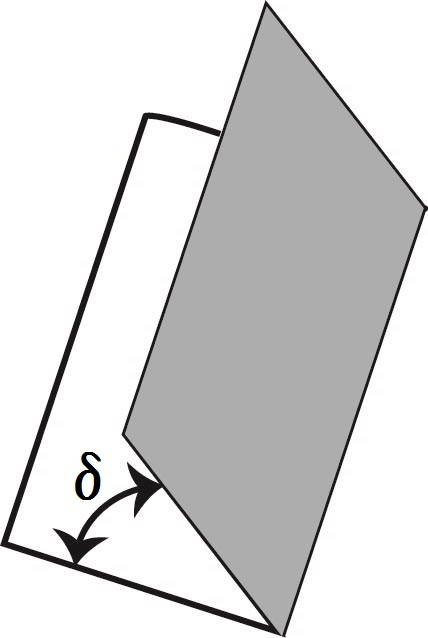
\includegraphics[scale=0.5]{gambarku/delta.jpg}}
	\caption{Sudut $\delta$} 
	\label{fig:sudut}
\end{figure}

Gambar \ref{fig:sudut} memperlihat sudut antara 2 bidang.
